\label {fs-acker-impl}

In the previous section, we introduced a general schema of the \tracker\ framework. In this section, we deepen into its implementation details. We describe and explore the properties of the tracking agent that produces the bound notifications. After that, the technique to achieve consistent notifications order is detailed. Distributed implementation of the tracking agent concludes this part.

\subsection{Bound guarantees}

As we stated earlier, each process sends to tracking agent the SND and RCV reports about each sending or receiving event $e = <action,m>$:
\begin{enumerate}
    \item $action$: send or receive.
    \item $pred(m)$: the result of applying a substream predicate.
    \item process (or {\em segment}) identifier.
\end{enumerate}

The tracking agent aggregates this information into the table illustrated in Table~\ref{tracker-table-simple}. Tracking agent builds for each predicate an indicator if a {\em graph segment} contains in-flight elements satisfying the predicate. Segments are subgraphs that incapsulate cycles. EOS that ensures soft substream end notifications can be sent for a subgraph if all upstream subgraphs do not contain the corresponding elements. The substream ends for the whole graph if all segments do not contain elements satisfying the prodicate~\footnote{Data source should also guarantee that it will not spawn any elements from this substream}. Therefore, the soft bound notifications for predicates $h(x)$ and $z(x)$ should be generated.

\begin{table}[htbp]
\caption{\tracker\ table: a general example}
  \label{tracker-table-simple}
  \centering
  \begin{tabular}{|c|c|c|>{\bfseries}c|} 
    \hline
    Notified & Predicate & Segment & Substream elements  \\ \hline \hline
    \multirow{2}{*}{\checkmark} & \multirow{2}{*}{h(x)} & A & No \\ \cline{3-4}
    & & B & No \\ \hline
    \multirow{2}{*}{} & \multirow{2}{*}{q(x)} & A & No \\ \cline{3-4}
    & & B & Yes \\ \hline
    \multirow{2}{*}{\checkmark} & \multirow{2}{*}{z(x)} & A & No \\ \cline{3-4}
    & & B & No \\ \hline
  \end{tabular}
\end{table}

A graph shown in Figure~\ref{fig:tracker-acker-comparison} illustrates the notion of segments. This graph has two segments: $A$ and $B$. Note that according to Table~\ref{tracker-table-simple}, the EOS for predicate $q(x)$ can be sent for a segment $A$, but not for a segment $B$. This behavior is similar to punctuations: notifications can be spawned earlier for the upstream processes.

\begin{figure}[htbp]
  \centering
  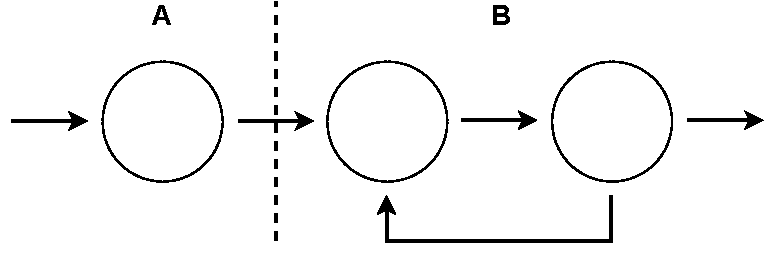
\includegraphics[width=0.3\textwidth]{pics/segments-example.pdf}
  \caption{Graph segmentation example}
  \label{fig:tracker-acker-comparison}
\end{figure}

There are several possible methods to build the indicator that the segment contains elements from a substream using the reports from processes. Our implementation uses the trick applied in Apache Storm to monitor the completeness of processing~\cite{apache:storm:acker}. 

Each report is labeled by a random number $X$, and this number is the same for the send action and the corresponding receive action. This trick makes a ``link'' in the reports chain and guarantees that there are no in-flight elements satisfying predicate $h(x)$ if and only if each report with $h(x)=1$ and a corresponding value $X$ is forwarded to the tracking agent exactly twice.

The latter condition can be easily checked by the tracking agent using XOR operation for all numbers received from the chain, which will turn into 0. The result of the XOR operation can accidentally become zero, but the probability of this event is controlled by the length of the random number $X$ so that it can be neglected in practice~\cite{apache:storm:acker}.

Figure~\ref{fig:tracker-reports} illustrates the reports with random numbers. The elements satisfying a predicate $h(x)$ flow through a dataflow. The first process generates an output and sends the SND report with $X=5$. The corresponding RCV report by the second process also has $X=5$ because this process receives the element from the first one. The second process sends a new element that satisfies $h(x)$ further, and the new SND report with $X=12$ is produced. The third operator receives this element and also produces an RCV report with $X=12$. If there are no more elements such that $h(x)=1$, then we can send EOS for the substream defined by $h(x)$ ends because {\em 5 XOR 5 XOR 12 XOR 12 = 0}. 

\begin{figure}[htbp]
  \centering
  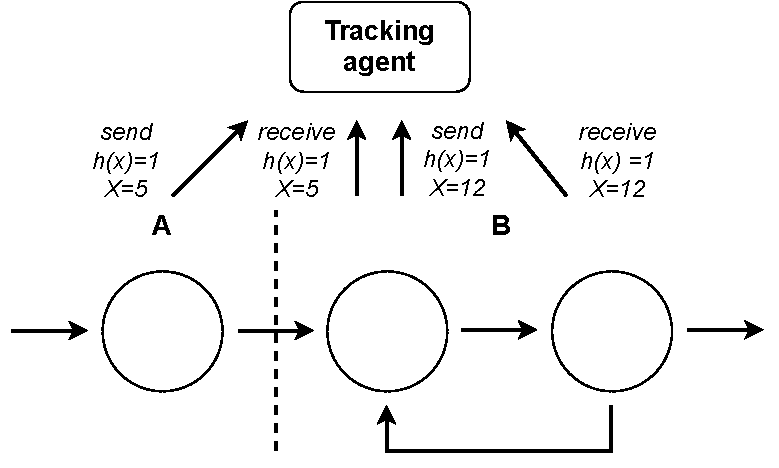
\includegraphics[width=0.3\textwidth]{pics/tracker-segments-example.pdf}
  \caption{Reports example}
  \label{fig:tracker-reports}
\end{figure}

Table~\ref{tracker-table-xor} illustrates the actual \tracker\ table for the mentioned technique. All reports from processes are grouped by the satisfying predicate and the segment. Random numbers from these reports are XORed into the result shown in columns {\em Segment XOR} and {\em XOR}. If the XOR value is equal to 0, then the tracking agent can send the EOS, providing the soft bound guarantee for the corresponding predicate.

\begin{table}[htbp]
\caption{\tracker\ table: an example with XORing technique}
  \label{tracker-table-xor}
  \centering
  \begin{tabular}{|c|c|c|>{\bfseries}c|>{\bfseries}c|} 
    \hline
    Notified & Predicate & Segment & Segment XOR & XOR  \\ \hline \hline
    \multirow{2}{*}{\checkmark} & \multirow{2}{*}{h(x)} & A & 000 & \multirow{2}{*}{000} \\ \cline{3-4}
    & & B & 000 & \\ \hline
    \multirow{2}{*}{} & \multirow{2}{*}{q(x)} & A & 000 & \multirow{2}{*}{110} \\ \cline{4-4}
    & & B & 110 & \\ \hline
    \multirow{2}{*}{\checkmark} & \multirow{2}{*}{z(x)} & A & 000 & \multirow{2}{*}{000} \\ \cline{3-4}
    & & B & 000 & \\ \hline
  \end{tabular}
\end{table}

As we described earlier, to ensure the firm notifications guarantee, one needs to block an input channel of a process if the element that does not belong to the substream arrives. After the EOS from the tracking agent arrives, the channel is unblocked.

Due to the XOR operation's commutative nature, we can optimize tracking agent incoming traffic by aggregating reports locally within the processes. For each process, we introduce a {\em local tracking agent} component. It serves as a mediator between the process and the global agent, buffering the outgoing reports and flushing them periodically. 

The flushing window is the parameter that allows us to balance between the notifications latency and the service traffic. Note that substreams last a finite time period by definition, so we assume that each process sends aggregated reports a constant number of times that does not depend on the number of substreams and processes. Therefore, the amount of extra network traffic for the reports is $O(||\Pi||)$, so the total estimation with the overhead on the notifications is $O(K||\Pi||)$.

% The amount of service network needed for \tracker\ is $O(||\Pi||)$, where $||\Pi||$ is the number of processes because all processes send reports to the tracking agent and the tracking agent sends notifications back to the processes. Therefore, traffic goes through a single agent without broadcasts between all processes. Further, we demonstrate how to make this agent distributed while keeping the same amount of extra traffic.

\subsection{Consistent notifications order}

To achieve consistent order of notifications, we need to define $t(x), x\in M$ such that the order on $t(x)$ coincides with the order of input elements. In this case, all reports that processes send to the tracking agent should be labeled by the $t(x)$. In turn, the tracking agent sends the EOS elements according to the order on $t(x)$.

Table~\ref{tracker-table-oder} illustrates the \tracker\ table in case of consistent notifications order. Column {\em min t(x)} indicates the minimal $t(x)$ among the elements that satisfy the corresponding predicate. The tracking agent sends notifications for the substream if the $XOR$ value is 0 and all substreams that contain elements with less {\em min t(x)} have finished (notifications has been produced). Therefore, notification for the substream defined by the predicate $h(x)$ is not sent until the notification for the predicate $q(x)$ is generated. 

\begin{table}[htbp]
\caption{\tracker\ table: an example with consistent notifications order}
  \label{tracker-table-oder}
  \centering
  \begin{tabular}{|c|c|>{\bfseries}c|c|} 
    \hline
    Notified & Predicate & min t(x) &  XOR  \\ \hline \hline
    \multirow{2}{*}{waits for q(x) finish} & \multirow{2}{*}{h(x)} & \multirow{2}{*}{5} & \multirow{2}{*}{000} \\
    & & & \\ \hline
    \multirow{2}{*}{} & \multirow{2}{*}{q(x)} & \multirow{2}{*}{4} & \multirow{2}{*}{110} \\
    & & & \\ \hline
    \multirow{2}{*}{\checkmark} & \multirow{2}{*}{z(x)} & \multirow{2}{*}{1} & \multirow{2}{*}{000} \\
    & & & \\ \hline
  \end{tabular}
\end{table}

If input elements arrive through a single node, $t(x)$ can denote the monotonic system time of the element $x$ arrival. If there are multiple source processes, one can use time oracle agent~\cite{10.14778/3055330.3055335} as a service for generation a monotonic sequence of unique timestamps. However, in this case, there is a need to manage one more subsystem.

A simple technique to build $t(x)$ without extra agents bases on systematic synchronization of the system clocks. Assume that clock differences are no more than some fixed $\delta$, which we reference as synchronization slack. Let $\tau(x)$ be precise physical time of input data item $x$ arrival, and $s(x)$ be local system time of the source node where $x$ arrived. The true order of events $\tau(d_1) > \tau(d_2)$ coming from different sources can be sometimes restored by their system timestamps $s(d_1)$ and $s(d_2)$. If these timestamps differ more than time synchronization slack, then the order is clear: $s(d_1) > s(d_2) + \delta \Rightarrow \tau(d_1) > \tau(d_2)$.

This fact allows us to define $t(x)$ such that $t(x) = [s(x) / \delta]$. This way we make $t(x)$ less precise, but this trick gives us an ability to compare global time associated by different source nodes. If $t(x_1)$ is greater by one than the $t(x_2)$ then their order is defined even if they arrived from different source nodes:  $t(x_1) > t(x_2) + 1 \Rightarrow \tau(x_1) > \tau(x_2)$. Therefore, the order on $t(x)$ coincides with the order of input elements, so it is suitable for the defined problem. Here is the summary of the mechanism that ensures consitent order notifications:
\begin{enumerate}
    \item On input item arrival, source node gets the system timestamp
    \item The system timestamp is shrunk up to synchronization slack (practically we achieve 10ms slack)
    \item Each report for the tracking agent is labeled by the result of $t(x)$
    \item Tracking agent sends bound notifications according to the order on $t(x)$
\end{enumerate}

\subsection{Distributed tracking agent}

As the tracking agent accumulates all the service traffic from the entire system, it may become a bottleneck. To deal with this problem, we introduce a distributed version of the tracking agent.

A straightforward approach is to partition predicates between the shards of the tracking agent. For example, one shard can handle all reports for the predicate $h(x)$, while the second all reports for the predicate $q(x)$. In this case, processes need to discover which shard is responsible for a predicate. Note that the network traffic complexity remains the same $O(K||\Pi||)$ because each process sends each report to only a single shard depending on the predicate.

The main problem regarding this approach is to enforce the consistent notifications order. Centralized agent sends EOS through the FIFO network channels, so the EOS elements for the same processes cannot be reordered. There can be a race between EOS from various shards due to asynchronous network channels in the distributed case.

A simple solution for this issue is on each EOS from some shard, wait for EOS from all other shards, but with greater $t(x)$. For example, if a process receives EOS for some predicate with $min t(x) = 3$, then it needs to wait until receiving EOS with $t(x) > 3$ from all other shards to produce the notification. However, this method can increase the latency between the substream end and the notification providing.

We employ the vector clock algorithm to mitigate latency overhead. Each process either periodically sends its system time to all tracking agent shards. In turn, tracking agents also periodically sends the minimal vector among the in-flight elements. Therefore, if a process receives EOS for some predicate with $min t(x) = 3, vec=[0,4,1]$, then it needs to wait until receiving of vectors component-wise greater than $[0,4,1]$ from all shards to produce the notification.

The vector clock introduction increases the service traffic but allows to eliminate bottleneck from the system. The service traffic complexity remains the same, but the $O$ factor increases. In the experimental section, we will study how significant is this increase.

% To make our system tolerant to the time difference between sources, we systematically synchronize the system clocks of them. We assume that clock differences are no more than some fixed $\delta$, which we reference as synchronization slack.

% \subsection{Elements ordering}
% In Section~\ref{sec:acker-analysis}, we have introduced the notion of \textit{global time}, without details of its practical implementation. One can use time oracle agent~\cite{10.14778/3055330.3055335} to generate a monotonic sequence of unique timestamps. However, in this case, the system will have a single point of failure. 

% To make our system tolerant to the time difference between sources, we systematically synchronize the system clocks of them. We assume that clock differences are no more than some fixed $\delta$, which we reference as synchronization slack.

% Let $\tau(d)$ be precise physical time of input data item $d$ arrival, and $s(d)$ be local system time of the source node where $d$ arrived. The true order of events $\tau(d_1) > \tau(d_2)$ coming from different sources can be sometimes restored by their system timestamps $s(d_1)$ and $s(d_2)$. If these timestamps differ more than time synchronization slack, then the order is clear: $s(d_1) > s(d_2) + \delta \Rightarrow \tau(d_1) > \tau(d_2)$.

% This fact allows us to define \textit{global time} slots $gt(d)$ such that $gt(d) = [s(d) / \delta]$. This way we make global time less precise,  on one hand but this trick gives us ability to compare global time associated by different source nodes on the other. If global time of an item $d_1$ is greater by one than the global time of some other element $d_2$ then their order is defined despite the source nodes associated their labels:  $gt(d_1) > gt(d_2) + 1 \Rightarrow \tau(d_1) > \tau(d_2)$. This property forms a basis of our guarantees mechanism. Here is the summary of labeling mechanism:
% \begin{enumerate}
%     \item On receiving of input item, source node gets the system timestamp
%     \item The system timestamp is shrunk up to synchronization slack (practically we use 10ms)
%     \item The item is labeled by the result \textit{global time} and this label is sent to \tracker\ agent
% \end{enumerate}

% \subsection{Metadata aggregation}
% \tracker\ agent has interface similar to Storm \acker, in a way that it receives \textit{ack} messages (\textit{global time} together with random \textit{ack value}) and subscribe/unsuscribe messages that is used to manage list of notifications subscribers. 

% However, the \tracker\  interface has several distinctions. Firstly, \textit{ack} messages are extended with a \textit{segment} label that is needed to provide dataflow-local notifications. Secondly, data sources should send special messages called \textit{heartbeats} that contain \textit{global time}. It promises that the source will not generate elements with lower or equal \textit{global time}. These messages allow \tracker\ to send notifications even if some sources did not produce records with a specific \textit{global time} due to low traffic. 

% \begin{algorithm}
% \caption{\tracker\ implementation sketch}
% \label{tracker_algo}
% \begin{algorithmic}[1]
% \State $inputs \leftarrow configured\_inputs;$ 
% \State $subscribers \leftarrow configured\_subscribers;$
% \State $segments \leftarrow List[Segment]$
% \State $segmentChecksums \leftarrow Map[Segment, List[Int64]]$
% \State $segmentMinTime \leftarrow Map[Segment, GlobalTime]$
% \State $sourceHeartbeat \leftarrow Map[Source, GlobalTime]$
% \\
% \State \textbf{Upon} (segment, gt, ack\_val) $from \ in\in inputs$
% \Indent
%     \State $segmentChecksums[segment][gt] \gets $
%     \par\Indent\Indent$segmentChecksums[segment][gt] \bigoplus checksum$\EndIndent\EndIndent
%     \State $CheckMinTime$
% \EndIndent
% \\
% \State \textbf{Upon} (gt, source) $from \ in\in inputs$
% \Indent
%  \State $sourceHeartbeat[source] \leftarrow gt$
%  \State $CheckMinTime$
% \EndIndent
% \\
% \Procedure{CheckMinTime}{}
% \State $minHeartbeat \leftarrow sourceHeartbeat.values.min()$
% \For {$segment \in segments$}
% \State $checksums \gets segmentChecksums[segment]$
% \State $maxTime \gets min($
% \par\Indent\Indent$minHeartbeat,$\EndIndent\EndIndent
% \par\Indent\Indent$segmentMinTime[segment.inbound].min(),$\EndIndent\EndIndent
% \par\Indent$)$\EndIndent
% \State $time \gets segmentMinTime[segment]$
% \While{$time < maxTime$
% \par\Indent$\And checksums[time] = 0$\EndIndent
% \par}
% \State $time \gets time + 1$
% \EndWhile
% \If{$segmentMinTime[segment] < time$}
% \State $segmentMinTime[segment] \gets time$
% \For {$subscriber \in subscribers$}
% \State $subscriber.send(segment, time)$
% \EndFor
% \EndIf
% \EndFor
% \EndProcedure
% \end{algorithmic}
% \end{algorithm}

% Therefore, \tracker\ receives the following messages:
% \begin{itemize}
%     \item Ack message is a tuple of a \textit{global time}, \textit{segment}, and \textit{ack value} (random number)
%     \item Heartbeat message is a pair of a \textit{global time} and a source id.
%     \item (Un)Subscribe message
% \end{itemize}

% % On ack message the accumulator, associated with provided \textit{global time} is updated by the received \textit{ack value}. Due to commutation of xor operation the checksum change may contain either single ack or multiple acks xored to a single change. The heartbeat message from source guarantees that no more input items with such a \textit{global time} will be emitted by this front-end. Subscribe messages manage the list of notification receivers. 

% \tracker\ sends the following messages to subscribers:
% \begin{itemize}
%     \item \textit{Min segment time update} for time $t$ when no items with the \textit{global time} less or equal $t$ exists in the segment and all preceding segments are complete
%     \item \textit{Min global time update} for time $t$ when no items with the \textit{global time} less or equal $t$ exists in the system
% \end{itemize}

% \textit{Min time update for segment} is emitted and send to all subscribers when:
% \begin{enumerate}
%     \item the \textit{heartbeat} for this time is received from all source nodes;
%     \item accumulators for all \textit{global times} not greater than this time plus one\footnote{The condition from the previous section requires the completeness of the next global time segment to preserve the order of the input elements in the notifications stream} are nullified;
%     \item upstream segments for this \textit{global time} have already sent \textit{min time updates}.
% \end{enumerate}
% If accumulators for all segments of a certain \textit{global time} become zero, \tracker\ sends \textit{min global time update}. An implementation sketch of \tracker\ interface is shown in Algorithm~\ref{tracker_algo}.

% % \subsection{Centralized \tracker\ }

% % \tracker\ is implemented as an "actor" on a dedicated machine and is shared between all system workers. It encapsulates minimal times received from the system fronts and a cyclic buffer for storing tracked elements.

% % Cyclic buffer stores checksums keyed by elements Global Time windows. It stores values in a fixed size range starting from current Minimal Global Time window. \tracker\ applies received Ack messages checksum changes to the corresponding value stored in the buffer.

% % \tracker\ can tell that there will be no more elements in a specific Global Time window when two conditions are fulfilled: no fronts will emit any more elements within this Global Time window and the cyclic buffer stores zero for it. Every time \tracker\ receives Acks or Heartbeats, it checks these conditions. If there are any matching windows \tracker removes them from the beginning of the buffer and broadcasts an update with the last of the windows.

% % \begin{algorithm}
% % \caption{\tracker}
% % \begin{algorithmic}[1]
% % \Procedure{HandleAck}{$time, checksum$}
% % \State $checksums[time] \gets checksums[time] \bigoplus checksum$
% % \State $CheckMinTime$
% % \EndProcedure
% % \\
% % \Procedure{HandleHeartbeat}{$time$}
% % \State $heartbeat \gets time$
% % \State $CheckMinTime$
% % \EndProcedure
% % \\
% % \Procedure{CheckMinTime}{}
% % \State $time \gets previousMinTime$
% % \While{$time < heartbeat \And checksums[time] = 0$}
% % \State $time \gets time + 1$
% % \EndWhile
% % \If{$previousMinTime < time$}
% % \State $previousMinTime \gets time$
% % \State $SendMinTimeUpdate(time)$
% % \EndIf
% % \EndProcedure
% % \end{algorithmic}
% % \end{algorithm}

% % To prevent false Min Time Updates this implementation has two requirements on order of processing:

% % \begin{itemize}
% %     \item Initial Ack message emitted from front with an input element must be processed before the following Heartbeat message.
% %     \item When operator processes an incoming element Ack messages of elements produced must be processed before an Ack message for incoming element.
% % \end{itemize}

% % Ordering of messages per sender-receiver pair given to us by Akka framework fulfils these requirements.

% \subsection{Single node tracking agent}
% The naive version of the \tracker\ agent can be implemented as a single node agent. In this case, the logic directly follows the Algorithm~\ref{tracker_algo}. Though, due to the commutative nature of XOR operation, we are able to optimize \tracker\ incoming traffic by aggregating ack messages locally on worker nodes before sending them to the \tracker\ agent. For each worker node in the system, we introduce a \textbf{Local \tracker} component. It serves as a mediator between the node and the \tracker, buffering the outgoing ack and \textit{heartbeat} messages and flushing them periodically. The flushing window is the parameter that allows us to balance between the system latency and the service traffic. The optimal value of this parameter is defined by the execution graph topology and timing of particular operations.

% \tracker\ use the latest \textit{heartbeat} message for each source and aggregates ack messages within the same \textit{global time} window to a single ack message via XOR product. On a flush, Local \tracker\ sends these messages in an ordered batch: ack messages come in order of associated \textit{global time} and \textit{heartbeat} messages come after them.

% \subsection{Distributed tracking agent}

% As \tracker\ agent accumulates all the service traffic from the entire system, it may become a bottleneck. To deal with this problem, we introduce a distributed version of the \tracker\ agent. The challenge here is to support the ability of the user-defined code to emit elements of \textit{global time} greater than the current. Otherwise, the problem becomes trivial as we can shard the \tracker\ agent by the \textit{global time}, and all \tracker\ chains will use the same shard along their path and the completion of certain \textit{global time} is permanent. In this case, we can send \textit{min time update} based on information from a particular shard.

% If this is not the case and the user is allowed to spawn items with the time greater than the time of the input element, it is possible that already nullified \textit{global time} will become active again. In this case, we need to take into account all \tracker\ shards to send the \textit{min time update} event.

% We employ the vector clock algorithm to resolve this issue. Each worker machine either periodically sends its system time to all \tracker\ shards. The vector of observed worker times accompanies all \tracker\ notification events. The \tracker\ table is built on the \textit{min time update} event receivers side. Each row in this table is associated with the vector of worker times. All conditions in the list for accepting \textit{min time update} now check that the associated time vector is not less than the vector of compared time. For example, we need to check that all accumulators of the same segment become zero \textit{and} their vector is component-wise not greater than the current one.

% The vector clock introduction increases the service traffic but allows to eliminate bottleneck from the system. The service traffic complexity remains the same, but the $O$ factor increases. In the experimental section, we will study how big is this increase.

% % \subsection{Operation-level tracking}

% % Our tracking mechanism can be made granular, tracking different parts of pipeline in case of directed acyclic graphs. For this we enrich Global Times with a pipeline identifier and change \tracker\ to track each pipeline part checksums in a separate buffer and limit minimal time of a pipeline part with minimal times of pipeline parts incoming into it. These changes make it possible for \tracker\ to emit Minimal Time Update messages for pipeline parts.
